\subsection{Spulenpaar}
In diesem Versuchsteil wird das Magnetfeld eines Spulenpaars für unterschiedliche Spulenanstände in Abhängigkeit des Ortes der Sonde bestimmt.
Die beiden Spulen haben identische Parameter.
Hierfür wird der Anleitung \cite[]{man:v308} eine Windungszahl von $n = 100$, ein mittlerer Durchmesser von $D = \qty[]{125}{\mm}$ und eine 
Spulenbreite von $b = \qty[]{33}{\mm}$ entnommen.
Die beiden Spulen sind in Reihe geschaltet und haben dementsprechend eine identische Stromstärke $I$.
Um den Spulenabstand zu variieren, kann eine Spule verschoben werden, während die andere befestigt bleibt.
Es wird für die Spulenabstände \qty[]{24}{\cm}, \qty[]{12}{\cm} sowie \qty[]{6}{\cm} gemessen, wobei letzterer in etwa einer Helmholtz-Anordnung entspricht.
Je nach Spulenabstand werden unterschiedlich viele Messwerte zwischen und hinter dem Spulenpaar aufgenommen, wobei $x$ der Abstand vom 
rechten Rand der linken Spule zur Sonde in Abbildung \ref{fig:spulenpaar} ist.
Auch hier soll jeweils ein $x$-$B$-Diagramm für jeden Spulenabstand erstellt werden, vgl. Abschnitt \ref{sec:spulenpaar}.
Für die Messung des Magnetfeldes steht eine transversale Hall-Sonde zur Verfügung, die entlang einer oberhalb der Spulen montierten Schiene verschoben werden kann.
Auch hier muss auf die Orientierung der Sonde geachtet werden.
Sowohl an der Schiene als auch an der Befestigung für die Spulen ist jeweils ein Lineal, um den Abstand zwischen linker Spule und Sonde bzw. den Spulenabstand 
zu bestimmen.
Da die auf der linken Seite der Anordnung nicht richtig befestigt ist, wird sie festgehalten, um beim Verscheiben der Sonde Ungenauigkeiten zu reduzieren.



\begin{figure}[H]
    \centering
    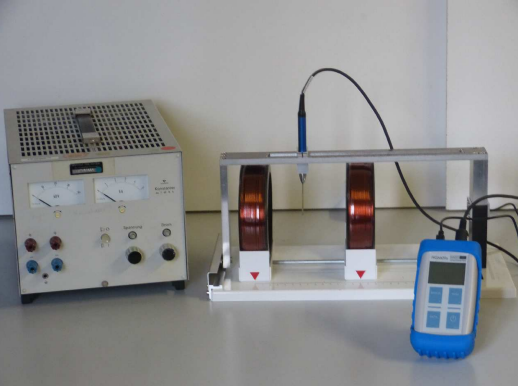
\includegraphics[height = 7cm]{abbildungen/spulenpaar.png}
    \caption{Versuchsaufbau zum Spulenpaar \cite[]{man:v308}.}
    \label{fig:spulenpaar}
\end{figure}
